\documentclass[conference]{IEEEtran}
\IEEEoverridecommandlockouts
% The preceding line is only needed to identify funding in the first footnote. If that is unneeded, please comment it out.
\usepackage{cite}
\usepackage{amsmath,amssymb,amsfonts}
\usepackage{algorithmic}
\usepackage{graphicx}
\usepackage{textcomp}
\usepackage{xcolor}
\def\BibTeX{{\rm B\kern-.05em{\sc i\kern-.025em b}\kern-.08em
    T\kern-.1667em\lower.7ex\hbox{E}\kern-.125emX}}
\begin{document}

\title{Climate Change Prediction with Machine Learning\\
}

\author{
\IEEEauthorblockN{Wooyoung Chung}
\IEEEauthorblockA{\textit{San Jose State University} \\
\textit{MS AI}\\}
\and
\IEEEauthorblockN{Mahavir Chandaliya }
\IEEEauthorblockA{\textit{San Jose State University} \\
\textit{MS CMPE}\\}
\and
\IEEEauthorblockN{Jiahong Zhan }
\IEEEauthorblockA{\textit{San Jose State University} \\
\textit{MS AI}\\}
\and
\IEEEauthorblockN{Bhavana Gangula}
\IEEEauthorblockA{\textit{San Jose State University} \\
\textit{MS CMPE}\\}
}

\maketitle

\begin{abstract}
Debate over climate change is contentious, particularly in the US, where many people reject the idea that human activity is causing it. It is critical to understand what causes the warming to better combat it because the consequences are predicted to be severe, including a mass extinction of marine life and frequent extreme weather events. The first challenge in this study is how to build trustworthy statistical models based on the collected climate data from the past 3 years and precisely capture temperature. We evaluated the performance of several widely used machine learning algorithms on our data, including Support Vector Machine, Logistic Regression and Neural Networks in order to build the model for confirming temperature change and identifying the contributing factors. The result should be assessed using numerals that takes into account a variety of additional factors, such as the highest and lowest possible temperatures, the highest and lowest pressures at sea level, the humidity, the visibility, the average wind speed, the maximum sustained wind speed, fog, and other variables.
\end{abstract}

\begin{IEEEkeywords}
component, formatting, style, styling, insert
\end{IEEEkeywords}

\section{Introduction}
With the rise of big data, powerful supercomputers with Graphics Processing Units (GPU), and scientific interest in new methods, the beginning of the 21st century turned out to be an important time in the history of machine learning [1]. However, the last few years, with their huge increases in data volume and computer power, are seen as the golden age of artificial intelligence and machine learning.
Many thematic articles [2–4] give detailed reviews of machine learning algorithms, which are the most important type of AI method in atmospheric science. In these books, you can find information about many methods and how they are grouped. Scientists who study the atmosphere found that supervised learning was the most interesting group of techniques. This is because it is the group that has been written about the most in recent papers in the field. If you have some data that has been labeled, you can use it as a training set to build a function that maps inputs to outputs. That function can be used to test the model on a different dataset called "testing one." If the results are good, it can be used in any classification or regression application. Methods like Decision Trees, Random Forest (RF) or XGBoost (XGB), Artificial Neural Networks (ANN), Deep Learning (DL), and Support Vector Machine (SVM) are in this group. On the other hand, in unsupervised learning, algorithms don't have labeled data to train on, so they have to figure out other ways to divide a dataset or reduce the number of dimensions.
The main purpose of this project is to give an overview of machine learning methods and how they are used in climate analysis. We show how machine learning techniques can be used as a new way to solve important and complicated problems in weather forecasting and the study of climate change over different time and space scales.Our team found a climate dataset from 2019 to 2021 for San Jose and from 1991 to 1995 for Madrid. We didn't want to show every part of each problem (for example, there are at least 13 different parts of climate change, but we did want to show the most important and interesting parts, which we found by reading scientific papers, and show that machine learning can be used successfully in climatology

\section{Methods}
This section will go over the process took in terms of data processing, data exploration, and model creation. 
\subsection{Data Preparation}
The dataset was obtained through combining two datasets from tutiempo.net- San Jose weather data containing the weather outcome of everyday from 2019 to 2021 san Jose and Madrid weather data containing the weather outcome of everyday from 1991 to 1995 Madrid. The cumulitive dataset size was 1989 with train-test split of 70-30.


The data used will include a variety of additional factors, such as the highest and lowest possible temperatures, the highest and lowest pressures at sea level, the humidity, the visibility, the average wind speed, the maximum sustained wind speed, fog, and other variables.


The data that were collected over the course of the three years do not correspond with one another. For instance, in a given year there may have been an average temperature and a humidity that corresponded to that, but there may not have been a wind speed that corresponded to that or fog at that time. In order to get the data ready for machine learning, we followed these steps to align the data. This was necessary because the algorithms that power machine learning cannot effectively deal with missing data points.
We performed the following pre-processing steps on the data: 
1) Data integration: combined the weather datasets of San Jose and Madrid 
2) Data cleaning: remove missing data 
3) Data reduction: remove unnecessary features 
4) Data transformation: create new features from current ones, convert the unit of temperature, and normalization.

\begin{table*}
\begin{tabular}{ |p{2cm}||p{2cm}|p{2cm}|p{2cm}|p{2cm}| p{2cm}|p{2cm}| }
 \hline
 \multicolumn{7}{|c|}{Data Mean/Max/Min}\\
  \hline
 Data & Temp (F) & hPA & Humidity & Visibility & AvgWindSpeed & Fog\\
 \hline

OriginalMean & 60.3 & 985.73 &61.19&13.67&13.67&0.0377
\\
OriginalMax & 89.78 & 1030.9 & 98.00 & 19.00 & 41.9 & 1
\\
OriginalMin & 28.94 & 934.00 & 12.00 & 0.60 & 0.60 & 0
\\
RainedMean & 55.15 & 979.65 &73.89&12.80&12.6&0.03
\\
RainedMax & 88.7 & 1026.4 & 97.00 & 16.1 & 41.9 & 1
\\
RainedMin & 36.32 & 934.2 & 12.00 & 2.10 & 1.10 & 0
\\
NotRainedMean & 61.66 & 987.20 & 58.36 & 13.88 & 9.62 & 0.039
\\
NotRainedMax & 89.78 & 1030.90 & 98.00 & 19.00 & 34.10 & 1
\\
NotRainedMin & 28.94 & 934.00 & 15 & 0.60 & 0.60 & 0
\\
\hline

\end{tabular}
\caption{Data Mean/Max/Min}
\label{MMM}
\end{table*}

\begin{figure}
\begin{center}
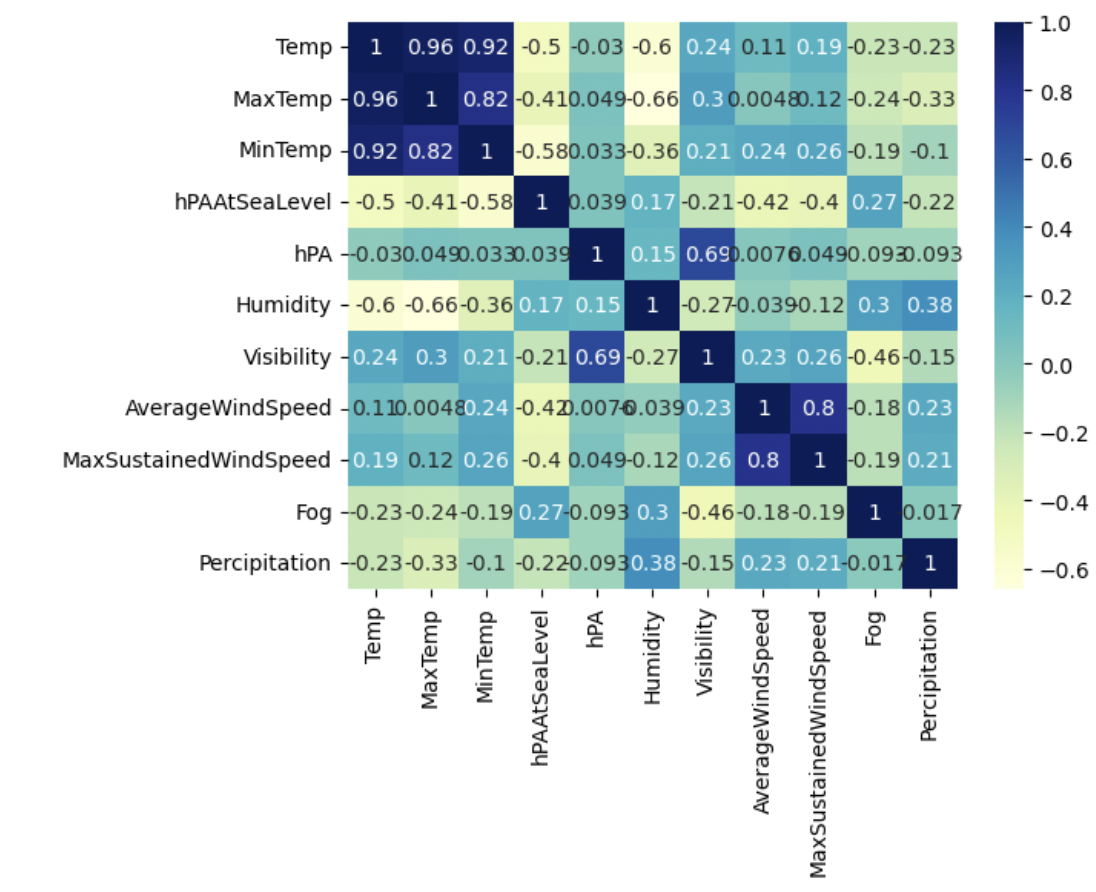
\includegraphics[width=.4\textwidth]{Heatmap.png}
\caption{Heatmap}
\label{Heatmap}
\end{center}
\end{figure}

\begin{figure}
\begin{center}
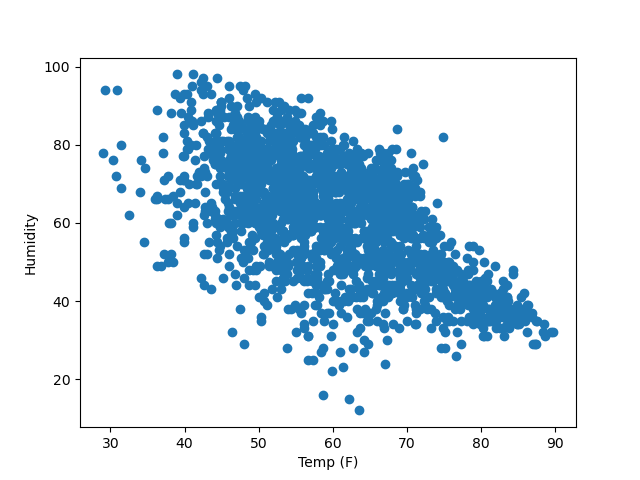
\includegraphics[width=.4\textwidth]{TempvsHumidity.png}
\caption{Temperature vs Humidity}
\label{TH}
\end{center}
\end{figure}

\subsection{Data Exploration}
Before creating the model, it is important to perform data exploration to check if there are any underlying pattern. From our analysis, we were successfully able to confirm the existence of pattern for predicting precipitation. The heatmap seen in Table \ref{Heatmap} show there are a lot of correlation between the features. Most notably, there are positive correlation between humidity and wind speeds.This infers that by high humidity and wind speeds leads to an increase in chance of precipitation. Furthermore, there are negative correlation between temperature, pressure at sea level, and visibility. This shows that there are the increase in temperature, pressure at sea level, and visibility leads to a decrease in the chance of precipitation. We can also see the pattern between features beyond just precipitation. Based on the heatmap Table \ref{Heatmap} and the scatter plot \ref{TH}, we can see that there is a negative correlation between temperature and humidity.

\subsection{Model Creation}
For implementation of Weather Prediction we tested various models on the dataset in order to come up with a best solution. We tested various models such as Support Vector Machine, Logistic Regression, Random Forest Classifier and Neural net. 

We further analyzed the learning using a 2-step learning approach and compared our results for various models. The goal here is to figure out a model that gives the best overall results for Weather Prediction and at the same time evaluate the results and outputs of other models. \\ \textbf{2-Step Learning}
There are two steps involved in learning for machine learning tasks:
\begin{enumerate}
\item $E_{out} \approx E_{in}$
\item $E_{in} \approx 0$
\end{enumerate}
where $E_{out}$ is the testing set error and $E_{in}$ is the training set error. Step 1 is important in ensuring that the model is good at predicting beyond the trained data, but also work well in the population data. To decrease the error bound between $E_{out} \approx E_{in}$, we must ensure that the dataset size is adequet, as increasing the training data size, will decrease the bound/likelihood of error. For our case, we set the acceptable error bound between $E_{out} \approx E_{in}$ to be 0.05. Step 2 is a optimization problem where we want to get the best model given our training data. This step can be done by creating a good model architecture to train on with good iteration. For our case, we considered a model to have "learned" as task to have error of 0.15\%.\\\textbf{Support Vector Machine}
SVM is a Supervised Machine Learning Algorithm used for classification and regression problems. It works by finding an optimal separation line called a hyperplane to accurately separate 2 or more different classes. The goal is to find the optimal hyperplane separation through training the linearly separable data with the SVM algorithm.
\textbf{Logistic regression}
A logistic regression model predicts a dependent data variable by analyzing the relationship between one or more existing independent variables. Logistic regression is easier to implement, interpret, and very efficient to train. 10 models were created using max iteration size of 1,000,000.
\textbf{Neural Networks}
A simple Neural network for classification is made up of a single hidden layer and a non-linear activation function. We have built a Neural Net with 4 layers of 12 neurons and an activation layer. Activation functions are mathematical equations or models that determine the output of a neural network. Activation functions also help normalize the output of each neuron to a range between -1, 0 and 1. We have used the Sigmoid Function that outputs the probabilities in the range of 0 to 1. 4 models were created using different epochs [1,000,2,000,3,000,10,000] with adam optimizer
\textbf{Random Forest}
Random forest is basically the combination of multiple individual decision trees to act as an ensemble. Ensemble learning can be defined as a paradigm whereby multiple learners are trained to solve the same problem. When it comes to classification using Random Forests, the idea is that the combination of outputs of mutually exclusive nodes will outperform any individual models which are then said to be the predicted output.

\begin{table}
\begin{center}
\begin{tabular}{|p{3cm}||p{1cm}|p{1cm}|p{2cm}| }
  \hline
 Model & Eout & Ein & Eout-Ein\\
 \hline
Logistic Regression & 0.1414& 0.0905 &0.0593
\\
Neural Network & 0.1324& 0.1034 & 0.0288
\\
Random Forest & 0.1206 & 0 & 0.1206
\\
Single Vector Machine & 0.1324& 0.1315 &0.0009
\\
\hline

\end{tabular}
\caption{2 Step Model Errors}
\label{2Step}
\end{center}
\end{table}

\section{Results}
This section will cover the analysis and juxtapose the different models created.
The error results of the models can be seen in Table \ref{2Step}. Based on the 2-step method of step 1 error of 0.05 and step 2 error of 0.15, we determined neural networks to be the best model for predicting precipitation.

Logistic regression and random forest was not considered to have learned the task.
For random forest, it was able to get no training error as the model is based around branch splitting on the training data. This result in a perfect accuracy, but have high deviance between $E_{in}$ and $E_{out}$. Logistic regression was also not considered to have learned due to the high deviance in $E_{in}$ and $E_{out}$. Logistic regression needs more data to reduce this deviance. 

Single vector machine and neural networks was considered to have learned the task by having $E_{out}-E_{in}$ to be below 0.05 and $E_{in}$ to be below 0.15. Although SVM did not have the best testing and training error, it had an extremely low $E_{in}$ and $E_{out}$, meaning that the model is very well generalized. SVM was able to also compete very well against neural networks in terms of $E_{out}$, demonstrating that a complex machine learning model is not always necessary to do good prediction. 

Neural network was considered to be the best model due having the highest accuracy that had acceptable $E_{out}-E_{in}$. The specific model that had the best performance was the model with epochs 10,000 which was surprising as the large epochs did not lead to the model being over fit.

\section{Conclusion}
In this work, we performed the supervised learning task of predicting precipitation given the weather condition. We first cleaned the dataset and explored it to confirm the existence of pattern. Then we created prediction models using various techniques; specifically, neural network, logistic regression, random forest, and single vector machine. From our results, we determined that neural network was the best technique on creating the model. Although the neural network model had the best performance, it is important to understand how close the other models were in juxtaposition to it. Random forest was able to gain better accuracy in terms of both testing and training dataset. Logistic regression gained a slight lead in the training accuracy. Single vector machine only had the training error difference of 0.03 despite being a much simpler model. This demonstrates that neural network is not always necessary in learning. For future work, we recommend trying recurrent neural network to see if it will improve on our basic neural network model. We recommend this because recurrent neural networks use nodes that create a cycle. This is useful as it allows for exhibiting temporal dynamic behavior that is good to train on time based data.




\begin{thebibliography}{00}
\bibitem{b1} Fradkov, A.L. Early History of Machine Learning. IFAC-PapersOnLine 2020, 53, 1385–1390. [http://doi.org/10.1016/j.ifacol.2020.12.1888]
\bibitem{b2} Mahesh, B. Machine Learning Algorithms—A Review; International Journal of Science and Research: Raipur, India, 2019. [http://doi.org/10.21275/ART20203995]
\bibitem{b3} Dhall, D.; Kaur, R.; Juneja, M. Machine Learning: A Review of the Algorithms and Its Applications. In Lecture Notes in Electrical
Engineering, Proceedings of the ICRIC, Jammu, India, 8–9 March 2019; Singh, P.K., Kar, A.K., Singh, Y., Kolekar, M.H., Tanwar, S., Eds.;
Springer International Publishing: Cham, Switzerland, 2020; pp. 47–63. [http://doi.org/10.1007/978-3-030-29407-65]
\bibitem{b4} Singh, A.; Thakur, N.; Sharma, A. A Review of Supervised Machine Learning Algorithms. In Proceedings of the 2016 3rd
International Conference on Computing for Sustainable Global Development (INDIACom), New Delhi, India, 16–18 March 2016,pp. 1310–1315.
\end{thebibliography}

\end{document}
